\documentclass[12pt]{article}

\usepackage[margin = 0.75in, paperwidth = 8.5 in, paperheight=11in]{geometry}
\usepackage{graphicx}

\newcommand\Mydiv[2]{%
$\strut#1$\kern.25em\smash{\raise.3ex\hbox{$\big)$}}$\mkern-8mu
        \overline{\enspace\strut#2}$}

\begin{document}

\title{Assignment 1}
\date{\today}
\author{Michael Cai}

\maketitle{}

\section{Exercise One}

Let $R(x) = \int_{0}^{x}\sqrt{1+t^2}dt$. Answer the following questions with justification.\\

(a) \textit{Evaluate $R(0)$ and determine if $R(x)$ is an even or an odd function.}\\
\\An integral is a tool to find the area bounded by the x-axis and the function represented by the integrand, which is bounded by the lower and upper limits of the integral. Therefore the integral of any function with the lower limit set equal to the upper limit would be equal to 0. This is because the area bounded would actually be a one-dimensional line. \\

Therefore \textbf{$R(0) = \int_{0}^{0} \sqrt(1+t^2) dt$ is equal to zero.} \\
\\
To determine if $R(x)$ is an even or an odd function, I refer to the theorem of \underline{Integrals of Symmetric Functions:}
\\
Suppose $f$ is continuous on $[-a,a]$: \\
(a) If $f$ is even $[f(-x) = f(x)]$, then $\int_{-a}^{a}f(x)dx = 2\int_{0}^{a}f(x)dx$ \\
(b) If $f$ is odd $[f(-x) = -f(x)]$, then $\int_{-a}^{a}f(x)dx = 0$ \\
\\*
To determine whether $R(x)$ is an odd or an even number, we must compare the outcomes of R given opposite inputs, x and -x. \\
For example, compare $R(1) = \int_{0}^{1} \sqrt{1+t^2}dt$ to $R(-1) = \int_{0}^{-1} \sqrt{1+t^2}dt$ which equals $-\int_{-1}^{0} \sqrt{1+t^2}dt$. \\
\\
(d) \textit{The graph clearly demonstrates the function $R(x)$:}\\
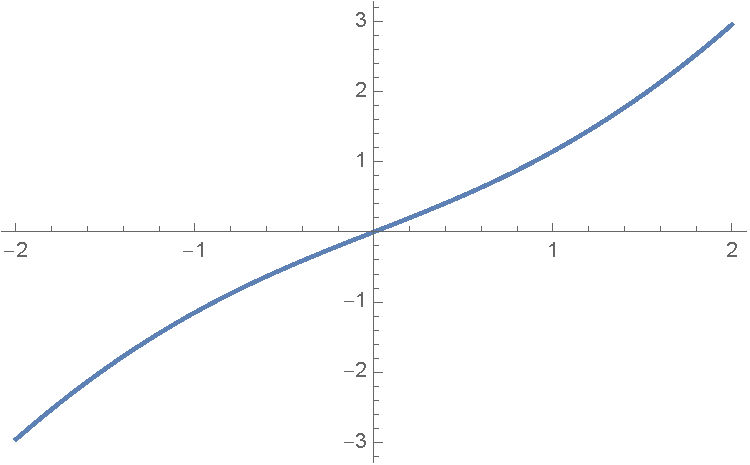
\includegraphics[width=.55\textwidth]{d_graph.pdf}

The integrand is a symmetric function, and thus even; however since $R(-1)$ causes the upper limit of the integral to be lower than the lower limit, you must evaluate $R(-1) = \int_{0}^{-1} \sqrt{1+t^2} dt $ as if it were $-\int_{0}^{1}\sqrt{1+t^2}dt$. Therefore $R(-1) = -R(1)$, and thus \textbf{$R(x)$ is an odd function.}
\\

\noindent (b) \textit{Is $R(x)$ increasing or decreasing?}\\
Because we have established that $R(x)$ is an odd function, we know that the value of $R(-x) = -R(x)$.\\
When $x>0$, $R(x)$ is increasing and positive because the integrand is increasing and positive.\\
Because $R(x)$ is an odd function, when $x<0$, $R(x)$ is decreasing and negative because the integrand is increasing and positive. 
Therefore \textbf{$R(x)$ is increasing} because as $x$ increases, $R(x)$ becomes less negative, and as it crosses 0, $R(x)$ becomes increasingly positive. \\

\noindent (c) \textit{What can you say about the concavity of $R(x)$?}\\
To find the concavity of $R(x)$ we must observe if $R''(x)$ is positive or negative. \\
By the Fundamental Theorem of Calculus Part 1, we know that $R(x) = \int_{0}^{x}f(t)dt \Rightarrow R'(x) = f(x)$, which further implies that $R''(x) = f'(x)$.\\
\\
$f'(x) = \frac{d}{dx}(\sqrt{1+x^2}) = \frac{1}{2}(1+x^2)^{-\frac{1}{2}}*2x$\\
= $x(1+x^2)^{-\frac{1}{2}}$\\
=$\frac{x}{\sqrt{1+x^2}}$ \\

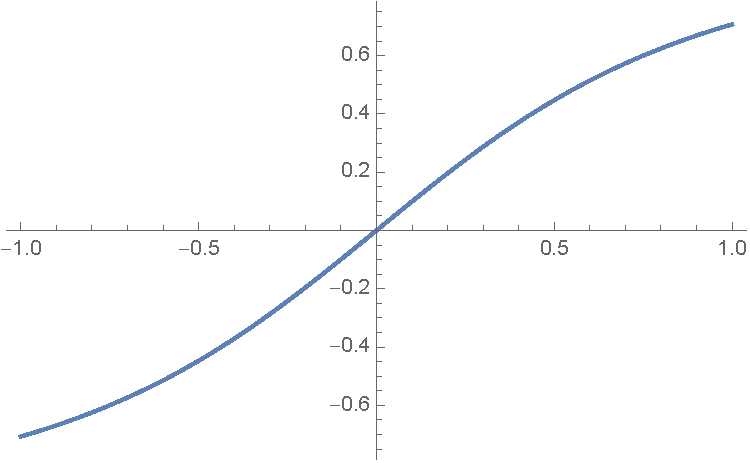
\includegraphics[width=.45\textwidth]{c_graph.pdf}

\noindent Because $f'(x)$ is positive at $[0,\infty]$ and negative at $[-\infty,0]$, $R(x)$ is \textbf{concave  up at} $[0,\infty]$ and \textbf{concave down at} $[-\infty,0]$.
\\~\\
(e) \textit{Find $\lim_{x\to\infty}\frac{R(x)}{x^2}$} \\
L'Hospital's rule states:\\
Suppose $f$ and $g$ are differentiable and $g'(x) \neq 0$ near a. \\
Then $\lim_{x\to\ a} \frac{f(x)}{g(x)} = \lim_{x\to\ a} \frac{f'(x)}{g'(x)}$ \\
$\Rightarrow \lim_{x\to\infty}\frac{R(x)}{x^2} = \lim_{x\to\infty}\frac{R'(x)}{2x} = \lim_{x\to\infty}\frac{\sqrt{1+x^2}}{2x}$ \\
As $x -> \infty$ 1 becomes an insignificant value and so $\lim_{x\to\infty}\frac{\sqrt{1+x^2}}{2x} \approx \frac{\sqrt{x^2}}{2x} = \frac{1}{2}$ \pagebreak

\section{Exercise Two} 
\textit{Order J,K,L, and 1 from smallest to largest. Justify your reasoning.} \\

\begin{figure}[!htb]
\minipage{0.32\textwidth}
  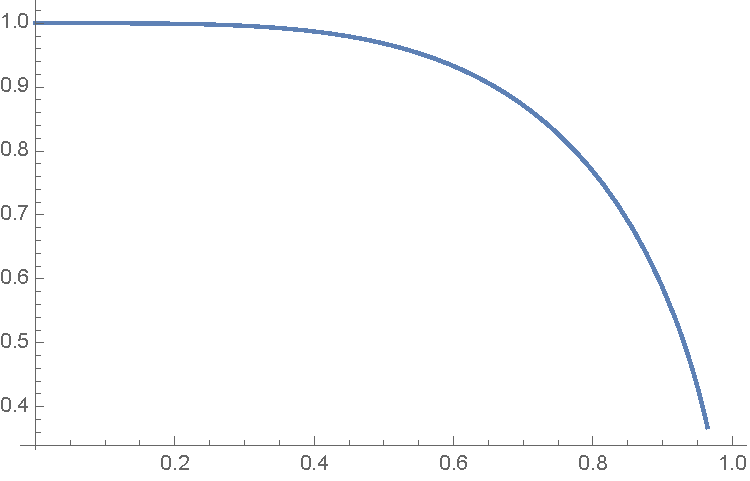
\includegraphics[width=\linewidth]{2J_graph.pdf}
  \caption{$J = \int_{0}^{1}\sqrt{1-x^4}$}
\endminipage\hfill
\minipage{0.32\textwidth}
  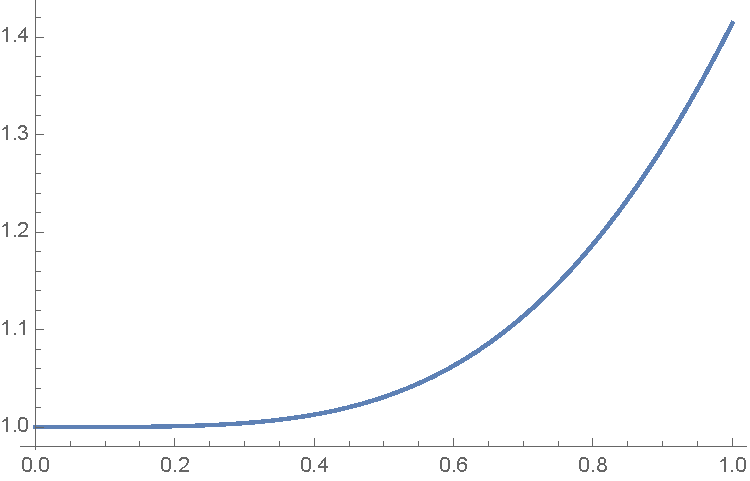
\includegraphics[width=\linewidth]{2K_graph.pdf}
  \caption{$K = \int_{0}^{1}\sqrt{1+x^4}$}
\endminipage\hfill
\minipage{0.32\textwidth}%
  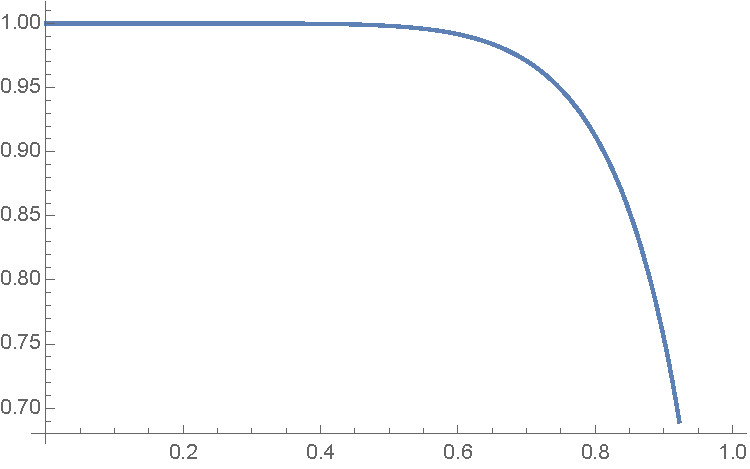
\includegraphics[width=\linewidth]{2L_graph.pdf}
  \caption{$L = \int_{0}^{1}\sqrt{1-x^8}$}
\endminipage
\end{figure}

Consider the domain $[0,1]$ given by $J$, $K$, and $L$. For an integral to equal 1, the area underneath the curve and above the x-axis must be equal that of a 1x1 unit square. \\
Both $J$ and $L$ bound less area than a unit square as evidenced by the graph. Given a number, x, between 0 and 1, higher powers of x will be much smaller than lower powers of x. Thus the integrand of $L$ is larger than the integrand of $J$ at all points from $[0,1]$ because the value at each point of the function is $\sqrt{1 - x^n}$ where the $n_J$ = 4, and the $n_L$ = 8. Therefore, $J < L$. \\

K is obviously larger than J, L, and 1 because the integrand's minimum value is 1 (at x = 0) and only increases as x approaches 1. Thus the area bounded by $K$ exceeds that of a 1x1 unit square.\\

\textbf{Therefore $J<L<1<K$}.

\section{Exercise 3}
Suppose $f(x)$ is a continuous function for all x and $\int_{0}^{x}f(t)dt = (\int_{x}^{1}t^2f(t)dt) + \frac{x^2}{4}+\frac{x^4}{8}+C$ for some constant C. \\~\\
(a) \textit{Find an explicit formula for $f(x)$. What is the main theorem you applied to find your answer?}\\~\\
By the Fundamental Theorem of Calculus Part 2, we know that if $F$ is the antiderivative of $f$ then $\int_{a}^{b}f(x)dx = F(b) - F(a)$. \\
Therefore, suppose $F$ is the antiderivative of $f$ and $G$ is the antiderivative of $t^2f(t)$. \\
Then $\int_{0}^{x}f(t)dt = \int_{x}^{1}t^2f(t)dt + \frac{x^2}{4} + \frac{x^4}{8}+C$\\
= $F(x) - F(0) = G(1) - G(x) + \frac{x^2}{4} + \frac{x^4}{8}+C$ \\~\\
If we take the derivative of both sides we get:\\~\\
$F'(x) = -G'(x) + \frac{x}{2} + \frac{x^3}{2}$ where $F'(x) = f(x)$ and $-G'(x) = -x^2f(x)$\\
Thus we have: $f(x) = -x^2f(x) + \frac{x}{2} + \frac{x^3}{2}$\\
= $x^2f(x) + f(x) = \frac{x}{2} + \frac{x^3}{2}$\\
= $f(x)(x^2+1) = \frac{x}{2} + \frac{x^3}{2}$\\
=$f(x) = \frac{\frac{x}{2} + \frac{x^3}{2}}{x^2+1}$ which simplifies to\\
=$f(x) = \frac{x}{2}$\\~\\
(b) \textit{Determine the value of C}.\\~\\
$\int_{0}^{x}f(t)dt = (\int_{x}^{1}t^2f(t)dt) + \frac{x^2}{4}+\frac{x^4}{8}+C$\\~\\
We plug in the $f(x)$ that we solved for:\\~\\
$\int_{0}^{x}\frac{x}{2} = \int_{x}^{1}t^2\frac{x}{2} + \frac{x^2}{4}+\frac{x^4}{8}+C$\\~\\

\noindent Let $u = t^2$ and thus $du = 2tdt$\\
Now we evaluate $\frac{t^2}{4}\bigg|$ on the LHS at 0 and 1 and $\frac{u^2}{8}\bigg|$ on the RHS at x and 1.\\~\\

\noindent Thus simplified we get, $\frac{x^2}{4} = \frac{1}{8}-\frac{x^2}{8} + \frac{x^2}{4}+\frac{x^4}{8}+C$\\
And therefore, $C = \frac{1}{8}$

\section{Exercise 4}
Evaluate the following indefinite and definite integrals using substitution. Clearly indicate your choice for $u$ and $du$. \\~\\
(a) $\int\frac{x+1}{x+2}dx$\\~\\
First we use long division to simplify the fraction. \\~\\
\Mydiv{x+2}{x+1} Which ends up giving $1 - \frac{1}{x+2}$\\
$= \int 1-\frac{1}{x+2}dx$ = $\int 1 - \int \frac{1}{x+2}$\\
Let $u = x+2$ and thus $du = 1dx$\\
$= \int 1 - \int \frac{du}{u}$\\
$= u - ln|u| + C = x + 2 - ln|x+2| + C$\\
$= x - ln|x+2| + C$\\~\\

\noindent(b) $\int \frac{1}{xln(x)ln(ln(x))}dx$\\
Let $u = ln(ln(x))$ and thus $du = \frac{1}{ln(x)} * \frac{1}{x} dx = \frac{1}{xln(x)} dx$\\
$= \int \frac{du}{u} = \int u^{-1} du = ln|u| + C$\\
$= ln|ln(ln(x))|+C$ \\~\\~\\~\\~\\

\noindent(c) $\int_{0}^{\pi/2} sin^n(x)cos(x)dx$ for $n \geq 0$\\
Let $u = sin(x)$ and thus $du = cos(x)dx$\\
Therefore the upper limit becomes $sin(\pi/2) = 1$ and the lower limit becomes $sin(0) = 0$\\
$= \int_0^{1} u^n du = \frac{u^{n+1}}{n+1} \bigg| 0$ to $1$\\
$=\frac{1}{n+1}$

\end{document}

